%% SECTION HEADER /////////////////////////////////////////////////////////////////////////////////////
\section{The \acs{sem}}
\label{sec:sem}

%% SECTION CONTENT ////////////////////////////////////////////////////////////////////////////////////

The general concept of the \ac{sem} is based on the idea of the \ac{fem}.
The similarity of both methods lies in the fact that the modelled domain is divided into non-overlapping finite elements, and external forces and arbitrary boundary conditions are imposed in the particular nodes.
The main difference between those methods is a choice of the shape function \( N=N(\xi )\), pictured in Fig.\ref{fig:shape}, which is interpolated by a Lagrange polynomial that passes through the element nodes.
The nodes are localized on the endpoint of an interval, \(\xi\in[-1,1]\), and the roots of the first derivative of Legendre polynomial P of degree \(p-1\):
\begin{eqnarray}
	(1-\xi^2)P'_{p-1}(\xi)=0.
	\label{eq:nodes}
\end{eqnarray}
The approximation of an integral over the elements is achieved according to \ac{gll} rule at points coinciding with the element nodes, 
and the weights \(w=w(\xi)\) calculated as:
\begin{eqnarray}
	{w(\xi)} = \frac{2}{p(p-1)(P_{p-1}(\xi))^2}.
	\label{eq:weight}
\end{eqnarray}

The shape functions and the weights for \ac{2d} or \ac{3d} elements are obtained by the Kronecker product of vectors of individual axes, denoted by \(\otimes\) as follows:
\begin{eqnarray}
	\begin{array}{rcl}
	N(\xi,\eta) & = & N(\xi)\otimes N(\eta),\\
	N(\xi,\eta,\zeta) & = & N(\xi)\otimes N(\eta)\otimes N(\zeta),
	\end{array}
\label{eq:shape_functions}
\end{eqnarray}
\begin{eqnarray}
	\begin{array}{rcl}
	w(\xi,\eta) & = & w(\xi)\otimes w(\eta),\\
	w(\xi,\eta,\zeta) & = & w(\xi)\otimes w(\eta)\otimes w(\zeta).
	\end{array}
	\label{eq:weights}
\end{eqnarray}
\begin{figure}[H]
	\begin{center}
		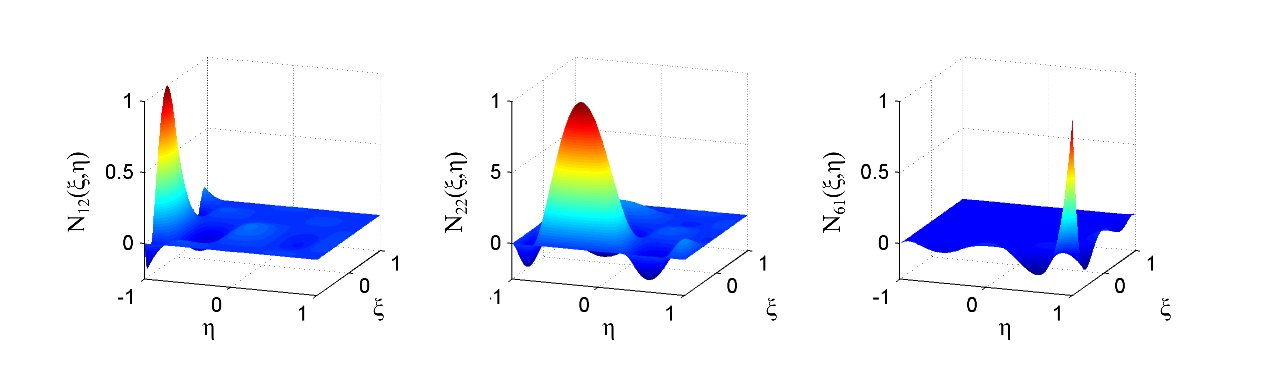
\includegraphics[width=0.95\textwidth]{Chapter_4/shape_function}
	\end{center}
	\caption{Shape functions for five order polynomial with \acf{gll} nodes.}
	\label{fig:shape}
\end{figure}

The elementary equations of motion are defined as:
\begin{eqnarray}
	\label{eq:motion}
	\textbf{M} \ddot{\textbf{d}} + \textbf{D} \dot{\textbf{d}} + \textbf{K} \textbf{d} = \textbf{F}_{ext},
\end{eqnarray}
where \textbf{d} is the displacement vector; \textbf{M}, \textbf{D} and \textbf{K} are the structural mass, damping and stiffness matrices, respectively; \textbf{F}$_{ext}$ is the external forces vector; \((\dot{\ })=\frac{\partial}{\partial t}\). 
The construction of the structural matrices is similar to the classical approach in \ac{fem}.

The most significant advantage of this method is the fast convergence of the equation of motion.
It is achieved for six nodes per wavelength, while at least fifteen nodes are needed in the case of linear elements in classic \ac{fem}~\cite{wee2017simulating}.
Moreover, the mass matrix is diagonal when the \ac{gll} approach is used, and solid or classic elements based on, the first order shear deformation theory is involved.
